% Font options: 10pm, 11pt, 12pt
% Align headings left instead of center: nocenter
\documentclass[xcolor=x11names,compress]{beamer}\usepackage[]{graphicx}\usepackage[]{color}
%% maxwidth is the original width if it is less than linewidth
%% otherwise use linewidth (to make sure the graphics do not exceed the margin)
\makeatletter
\def\maxwidth{ %
  \ifdim\Gin@nat@width>\linewidth
    \linewidth
  \else
    \Gin@nat@width
  \fi
}
\makeatother

\definecolor{fgcolor}{rgb}{0.345, 0.345, 0.345}
\newcommand{\hlnum}[1]{\textcolor[rgb]{0.686,0.059,0.569}{#1}}%
\newcommand{\hlstr}[1]{\textcolor[rgb]{0.192,0.494,0.8}{#1}}%
\newcommand{\hlcom}[1]{\textcolor[rgb]{0.678,0.584,0.686}{\textit{#1}}}%
\newcommand{\hlopt}[1]{\textcolor[rgb]{0,0,0}{#1}}%
\newcommand{\hlstd}[1]{\textcolor[rgb]{0.345,0.345,0.345}{#1}}%
\newcommand{\hlkwa}[1]{\textcolor[rgb]{0.161,0.373,0.58}{\textbf{#1}}}%
\newcommand{\hlkwb}[1]{\textcolor[rgb]{0.69,0.353,0.396}{#1}}%
\newcommand{\hlkwc}[1]{\textcolor[rgb]{0.333,0.667,0.333}{#1}}%
\newcommand{\hlkwd}[1]{\textcolor[rgb]{0.737,0.353,0.396}{\textbf{#1}}}%
\let\hlipl\hlkwb

\usepackage{framed}
\makeatletter
\newenvironment{kframe}{%
 \def\at@end@of@kframe{}%
 \ifinner\ifhmode%
  \def\at@end@of@kframe{\end{minipage}}%
  \begin{minipage}{\columnwidth}%
 \fi\fi%
 \def\FrameCommand##1{\hskip\@totalleftmargin \hskip-\fboxsep
 \colorbox{shadecolor}{##1}\hskip-\fboxsep
     % There is no \\@totalrightmargin, so:
     \hskip-\linewidth \hskip-\@totalleftmargin \hskip\columnwidth}%
 \MakeFramed {\advance\hsize-\width
   \@totalleftmargin\z@ \linewidth\hsize
   \@setminipage}}%
 {\par\unskip\endMakeFramed%
 \at@end@of@kframe}
\makeatother

\definecolor{shadecolor}{rgb}{.97, .97, .97}
\definecolor{messagecolor}{rgb}{0, 0, 0}
\definecolor{warningcolor}{rgb}{1, 0, 1}
\definecolor{errorcolor}{rgb}{1, 0, 0}
\newenvironment{knitrout}{}{} % an empty environment to be redefined in TeX

\usepackage{alltt}
%\documentclass[xcolor=x11names,compress,handout]{beamer}
\usepackage[]{graphicx}
\usepackage[]{color}
\usepackage{booktabs}
\usepackage{hyperref}
\usepackage{tikz}
\usepackage{multirow}
\usepackage{dcolumn}
\usepackage{bigstrut}
\usepackage{amsmath} 
\usepackage{xcolor,colortbl}
\usepackage{amssymb}
%\newcommand{\done}{\cellcolor{teal}#1}

%% Beamer Layout %%%%%%%%%%%%%%%%%%%%%%%%%%%%%%%%%%
\useoutertheme[subsection=false,shadow]{miniframes}
\useinnertheme{default}
\usefonttheme{serif}
\usepackage{Arev}
\usepackage{pdfpages}

\setbeamerfont{title like}{shape=\scshape}
\setbeamerfont{frametitle}{shape=\scshape, size=\normalsize}

\definecolor{dkblue}{RGB}{0,0,102}

\setbeamercolor*{lower separation line head}{bg=dkblue} 
\setbeamercolor*{normal text}{fg=black,bg=white} 
\setbeamercolor*{alerted text}{fg=red} 
\setbeamercolor*{example text}{fg=black} 
\setbeamercolor*{structure}{fg=black} 
 
\setbeamercolor*{palette tertiary}{fg=black,bg=black!10} 
\setbeamercolor*{palette quaternary}{fg=black,bg=black!10} 

\renewcommand{\(}{\begin{columns}}
\renewcommand{\)}{\end{columns}}
\newcommand{\<}[1]{\begin{column}{#1}}
\renewcommand{\>}{\end{column}}

\setbeamertemplate{navigation symbols}{} 
\setbeamertemplate{footline}[frame number]
\setbeamertemplate{caption}{\raggedright\insertcaption\par}

\setbeamersize{text margin left=5pt,text margin right=5pt}

%%%%%%%%%%%%%%%%%%%%%%%%%%%%%%%%%%%%%%%%%%%%%%%%%%


\title{Making Causal Critiques}
\subtitle{Day 5 - Constructive Critiques}
\author{Jonathan Phillips}
\IfFileExists{upquote.sty}{\usepackage{upquote}}{}
\begin{document}

\frame{\titlepage}

\section{Constructive Critiques}

\begin{frame}
\frametitle{Being Constructive}
\begin{itemize}
\item Effective critiques are essential to learning
\pause
\begin{itemize}
\item We have a scholarly obligation to point out errors in reasoning
\pause
\item We learn collectively by collaborating
\pause
\item We learn individually by thinking critically about others' work
\pause
\end{itemize}
\item There is no research project that cannot be improved
\end{itemize}
\end{frame}

\begin{frame}
\frametitle{Being Constructive}
\begin{itemize}
\item But criticism can also be used as a weapon
\pause
\begin{itemize}
\item To compete for attention/jobs
\pause
\item To discourage colleagues
\pause
\item To assert status/hierarchy/superiority
\pause
\item To destroy valuable research
\pause
\item To release our own frustrations
\end{itemize}
\end{itemize}
\end{frame}

\begin{frame}
\frametitle{Being Constructive}
\begin{itemize}
\item To avoid these risks, we must make our criticisms \textbf{constructive}
\pause
\begin{enumerate}
\item In terms of style
\pause
\item In terms of content
\end{enumerate}
\end{itemize}
\end{frame}

\section{Constructive Style}

\begin{frame}
\frametitle{Styles of Critique}
\begin{itemize}
\item Your task is to convince the author to \textit{improve} their work not to \textit{abandon} it
\pause
\item So they have to:
\begin{itemize}
\item Understand your comment
\pause
\item Not take it as a personal attack/become defensive
\pause
\item Have options for how to respond
\end{itemize}
\end{itemize}
\end{frame}

\begin{frame}
\frametitle{Styles of Critique}
\begin{itemize}
\item Always remember your critique might be wrong!
\pause
\begin{itemize}
\item You always know the data less well than the author
\pause
\item Recognize the inherent challenges and constraints of implementing the research
\pause
\end{itemize}
\item So phrase your comment in terms of 'as I understand your argument'
\pause
\item Or 'Could it be that something else is also happening?'
\end{itemize}
\end{frame}

\begin{frame}
\frametitle{Styles of Critique}
\begin{itemize}
\item \textbf{Be specific!} Which part of the research design is problematic?
\pause
\item \textbf{Be concrete!} Use an example/counterexample to communicate the risk
\pause
\item \textbf{Be objective!} We care about the research quality, not your personal opinion
\pause
\item \textbf{Suggest an alternative}
\end{itemize}
\end{frame}

\begin{frame}
\frametitle{Styles of Critique}
\begin{itemize}
\item Depersonalize criticism
\pause
\begin{itemize}
\item Instead of "you did it wrong...", refer to "in this type of research there is a risk..."
\pause
\item "I feel like there might be some readers who did not understand..."
\pause
\end{itemize}
\item If in doubt, use the feedback sandwich:
\pause
\begin{enumerate}
\item Something positive/encouraging
\item Critique
\item Something positive/encouraging
\end{enumerate}
\end{itemize}
\end{frame}

\begin{frame}
\frametitle{Styles of Critique}
\begin{itemize}
\item Finally:
\pause
\begin{itemize}
\item Is the comment really necessary?
\pause
\item If it is a minor issue, is there a better way to communciate it?
\pause
\item If you have not fully understood, take time to invest in understanding it before commenting
\end{itemize}
\end{itemize}
\end{frame}

\section{Constructive Content}

\begin{frame}
\frametitle{Strengthening Causal Arguments}
\begin{enumerate}
\item Multiple tests of theory
\pause
\item Multiple methods
\pause
\item Uncovering 'hidden' units
\pause
\item Heterogeneity tests
\pause
\item Placebo tests
\pause
\item Investigating Mechanisms
\end{enumerate}
\end{frame}

\begin{frame}
\frametitle{1. Multiple Tests}
\begin{itemize}
\item Learning requires testing theories with evidence
\pause
\item Competing theories have \textbf{multiple distinct implications}
\pause
\item We should test \textit{all} of these implications
\item "The dog that didn't bark"
\pause
\begin{itemize}
\item If a theory has multiple implications, and we find one of these did not occur in reality, we have evidence against our theory
\pause
\end{itemize}
\item \textbf{Critical tests}: Ideally we want to focus on those tests that 'separate' theories, telling us which one is true
\end{itemize}
\end{frame}

\begin{frame}
\frametitle{1. Multiple Tests}
\begin{itemize}
\item For example, Deaton argues poor health causes low economic status
\pause
\begin{itemize}
\item But the critique is of possible reverse causation: Low economic status causes poor health.
\pause
\end{itemize}
\item Additional tests to support his argument include:
\pause
\begin{enumerate}
\item Whether the relationship falls after retirement
\pause
\item Whether the relationship is weaker among women, who on average work fewer hours
\pause
\item Whether the relationship holds even for diseases which could easily be cured with more income
\end{enumerate}
\end{itemize}
\end{frame}

\begin{frame}
\frametitle{2. Multiple Methods}
\begin{itemize}
\item Our methodologies' assumptions are often impossible to test in quantitative data
\pause
\item But qualitative evidence can help justify our assumptions
\pause
\item This means using multiple (mixed) methods
\pause
\item These are all "Causal Process Observations" (Collier et al 2010)
\end{itemize}
\end{frame}

\begin{frame}
\frametitle{2. Multiple Methods}
\begin{itemize}
\item Examples of Causal Process Observations:
\pause
\begin{itemize}
\item What is the treatment assignment mechanism? Who decides when teachers get evaluated?
\pause
\item Is selection bias possible in the data? How was the dataset constructed?
\pause
\item Was randomization of a field experiment successful? We can interview people about the process, gather documents
\pause
\item Are there spillovers (violations of SUTVA)? We can conduct a survey and find out how people interacted
\pause
\item Is a regression discontinuity threshold enforced neutrally? Or was the threshold chosen to make sure a particular unit passed?
\pause
\item Can people sort/migrate across a discontinuity? We can use administrative data on migration rates to assess if these differences might be large enough to explain our results
\end{itemize}
\end{itemize}
\end{frame}

\begin{frame}
\frametitle{2. Multiple Methods}
\begin{itemize}
\item Nunn (2008) asks whether the slave trade explains underdevelopment in parts of Africa, using an instrumental variable for distance to the Americas
\pause
\item Qualitative evidence helps:
\pause
\begin{itemize}
\item To verify that slaves usually sailed from the nearest port, and not a different country
\pause
\item To inform the need for extra controls, eg. for legal system, natural resources
\pause
\item To identify the direction of the bias - reverse causation is less of a problem because he shows the richest ethnic groups were most affected by the slave trade
\pause
\item To argue in support of the exclusion restriction for the instrumental variable: that plantations were set up in the Carribean because of the climate, not because they were near the supply of slaves in West Africa
\end{itemize}
\end{itemize}
\end{frame}

\begin{frame}
\frametitle{3. Uncovering 'Hidden' Units}
\begin{itemize}
\item What if our sample size is small, there is no experimental option and selection bias is a concern? 
\pause
\item One strategy is to identify more units:
\pause
\begin{itemize}
\item Those units are often 'hidden', either because we did not think about them or there is no data on them initially
\pause
\item We can expand our dataset and adjust our research question
\pause
\item For example, John Londregan's seminar 'uncovered' non-trading product-country pairs to provide another source of variation to explain
\end{itemize}
\end{itemize}
\end{frame}

\begin{frame}
\frametitle{3. Uncovering 'Hidden' Units}
\begin{itemize}
\item Lewis (2016) wanted to ask whether ethnicity affected the formation of rebel groups
\pause
\item But there is a selection/survival bias in the data - we only have data on the groups that \textit{succeeded}
\pause
\item She collected data from Uganda on \textit{all} rebel groups
\pause
\begin{itemize}
\item Expanding the sample from 1-4 (in most datasets) to 15
\pause
\item Showing that ethnicity does \textit{not} affect rebel group formation, but may affect their success
\end{itemize}
\end{itemize}
\end{frame}

\setbeamercolor{background canvas}{bg=}
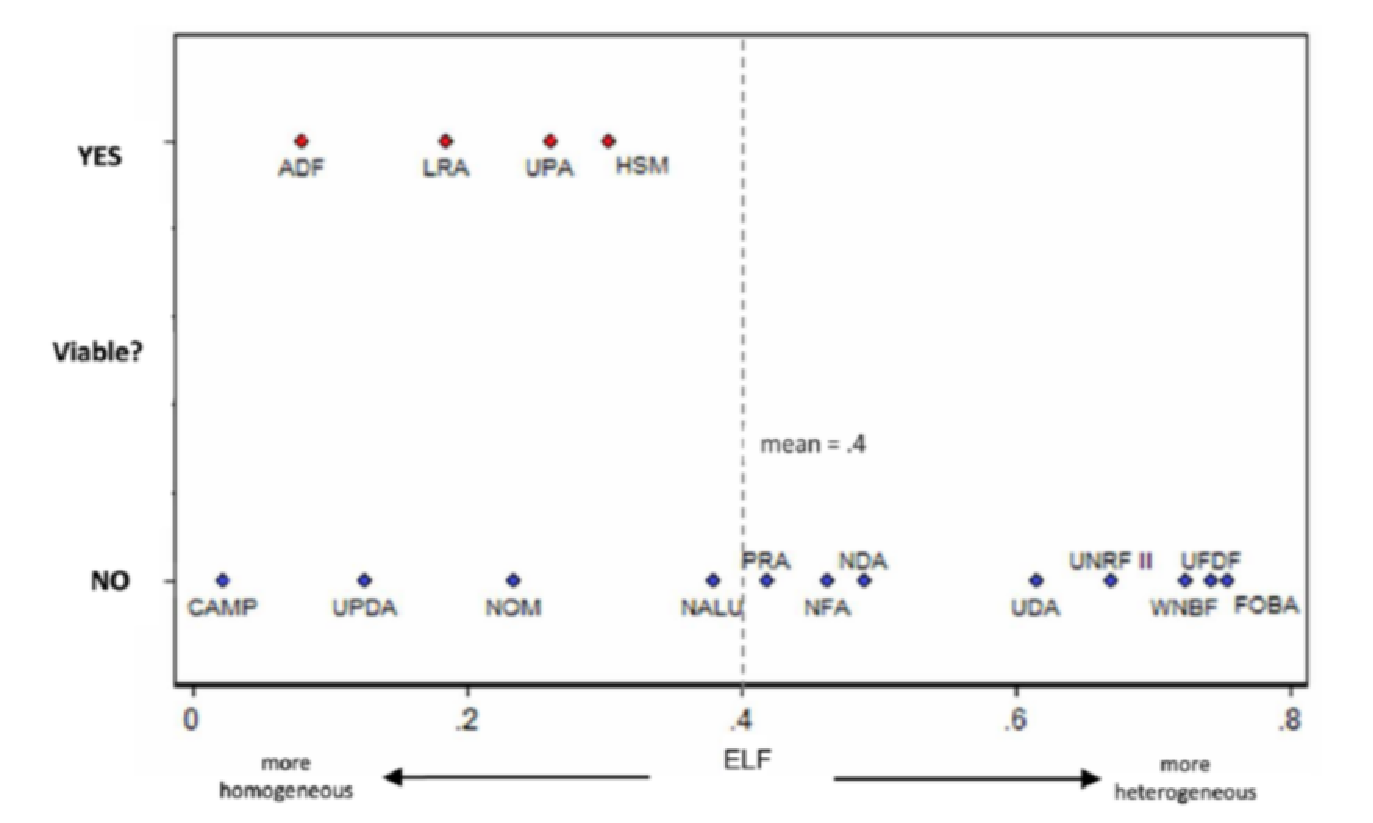
\includepdf[pages={1}]{Lewis_rebels.pdf}

\begin{frame}
\frametitle{4. Heterogeneity Tests}
\begin{itemize}
\item Sometimes the implications of theory are very precise
\pause
\item Treatment is likely to have affected subgroups to different degrees
\pause
\item We can use heterogeneity tests to disaggregate the effect to each subgroup and compare
\end{itemize}
\end{frame}

\begin{frame}
\frametitle{4. Heterogeneity Tests}
\begin{itemize}
\item For example, Ferraz and Finan (2008) ask how random audits affect corruption rates
\pause
\item They find that audits significantly reduce corruption
\pause
\item Their theory is that this is produced by 'electoral accountability'   
\pause
\item They provide evidence for this specific theory by:
\pause
\begin{itemize}
\item Subsetting the data to only those municipalities with local radio stations which broadcast the findings of corruption and showing the effect is much \textit{stronger}
\pause
\item Subsetting the data to only those municipalities with mayors in their first-term who face re-election incentives, showing corruption is \textit{lower}
\pause
\end{itemize}
\item What other theory would be consistent with \textit{all} of this evidence?
\end{itemize}
\end{frame}

\begin{frame}
\frametitle{5. Placebo tests}
\begin{itemize}
\item Our theory has very precise implications, and we normally test the 'positive' version
\pause
\item But we can also test the 'non-predictions' of our theory, when there should \textit{not} be an effect
\pause
\item If we found an effect where there should \textit{not} be one, we might think something is weird in our data/methodology and have less confidence in our main result
\end{itemize}
\end{frame}

\begin{frame}
\frametitle{5. Placebo tests}
\begin{itemize}
\item For example, with a regression discontinuity on close elections we expect a 'jump' effect when elections are tied (winning margin=0)
\pause
\item We expect there \textit{not} to be a 'jump' effect when winning margin=10\%
\pause
\item So we can apply our regression discontinuity again and measure the effect at winning margin=10\%
\pause
\item If we still find an effect, there might be something wrong with our data/method
\end{itemize}
\end{frame}

\begin{frame}
\frametitle{5. Placebo tests}
\begin{itemize}
\item The same with difference-in-differences
\pause
\item If we were estimating the effect of a treatment that applied to some units on 5th August 2012, we expect no effect on 3rd July 2009
\pause
\begin{itemize}
\item Or on 4th August 2012
\pause
\item Or on 6th August 2012
\pause
\end{itemize}
\item The more tightly the data are consistent \textit{only} with your theory, the more credible is your theory
\end{itemize}
\end{frame}

\begin{frame}
\frametitle{5. Placebo tests}
\begin{itemize}
\item Placebo tests also work for small-N studies (Glynn and Ichino 2012)
\pause
\item We want to assess the effect of presidentialism on reducing party cohesion
\pause
\item A good comparison is between the USA (presidential) and Canada (parliamentary)
\pause
\item But we also gain confidence if we can show that other similar parliamentary systems have cohesive parties (Britain, Australia, etc.)
\end{itemize}
\end{frame}

\begin{frame}
\frametitle{6. Mechanisms}
\begin{itemize}
\item Often we talk as though we are testing 'treatments'
\pause
\begin{itemize}
\item But that leaves an empty black box between treatment and outcome
\pause
\end{itemize}
\item Really we want to test \textbf{theories}, which include a clear mechanism connecting the treatment and the outcome
\pause
\item To show that a specific theory is operating, we want to trace every step of the mechanism
\end{itemize}
\end{frame}

\begin{frame}
\frametitle{6. Mechanisms}
\begin{itemize}
\item For example, multiple studies show a clear treatment effect: high ethnic diversity reduces public goods provision
\pause
\begin{itemize}
\item But these studies had \textit{no theory}
\pause
\end{itemize}
\item Habyarimana et al (2007) asked "why?"
\pause
\begin{itemize}
\item Preferences
\item Technology
\item Strategy selection
\pause
\end{itemize}
\item They designed laboratory games to test exactly each mechanism
\pause
\item Eg. To test if there is an ethnic 'technology' that helps co-ethnics, they asked Ugandans to find a specific person in a neighbourhood, and paid them a reward if they did
\pause
\begin{itemize}
\item Co-ethnics found their target 43\% of the time, non-co-ethnics only 28\% of the time
\end{itemize}
\end{itemize}
\end{frame}

\begin{frame}
\frametitle{6. Mechanisms}
\begin{itemize}
\item Process Tracing is one way of demonstrating which mechanism connected the treatment and the outcome 
\pause
\item Within-case analysis
\pause
\item We turn our single case into \textbf{multiple} observations - usually over time
\pause
\item We test if those process observations are consistent with our theory
\pause
\item But what happened to counterfactuals here? 
\pause
\item We’re substituting assumptions/theory for a counterfactual
\pause
\item Provides evidence for our specific case; generalization is hard
\end{itemize}
\end{frame}

\begin{frame}
\frametitle{6. Mechanisms}
\begin{itemize}
\item Brady (2004) provides an example of a type of process tracing to evaluate the plausibility of a difference-in-differences research design
\pause
\item Difference-in-differences analysis suggested media announcements that Al Gore won Florida in 2000 caused 10,000 Gore voters to stay at home, allowing Bush to win.
\pause
\item But:
\pause
\begin{itemize}
\item There were only 10 minutes until the polling stations closed
\pause
\item Only about 20\% would have heard the announcements
\pause
\item Around half were Bush voters, who may also have stayed home
\pause
\item Voters still had a reason to vote for other offices
\pause
\end{itemize}
\item Brady estimates that at most 224 people did not vote due to the media announcements
\end{itemize}
\end{frame}

\end{document}
 % effects of causes vs. reverse
